%%%%%%%%%%%%%%%%%%%%%%%%%%%%%%%%%%%%%%%%%%%%%%%%%%%%%
%
% Plantilla Anteproyecto de Grado
% Leonel Muñoz Cedano (c) 2017
% MCIC - Ingeniería de Software
%%%%%%%%%%%%%%%%%%%%%%%%%%%%%%%%%%%%%%%%%%%%%%%%%%%%%

%%%%%%%%%%%%%%%%%%%%%%%%%%%%%%%%%%%%%%%%%%%%%%%%%%%%%
%
% Nombre del proyecto: 
% Autores: 
%
%%%%%%%%%%%%%%%%%%%%%%%%%%%%%%%%%%%%%%%%%%%%%%%%%%%%%

%\documentclass[11pt,letterpaper,oneside]{article}
\documentclass[11pt,letterpaper,oneside]{article}

% Inclusion de paquetes
\usepackage[utf8x]{inputenc} % Tildes
\usepackage{url}

%%%% Inicio - Tipo letra Arial - por defecto es (Times New Roman) %%%
\usepackage[T1]{fontenc}
\usepackage{uarial}
\renewcommand{\familydefault}{\sfdefault}
%%% fin - Tipo de letra %%%%

%%%%  inicio - Formato a las secciones del documento %%%%%%%
\usepackage{titlesec}
\titleformat{\section}[hang]{\bfseries} {\Large\thesection}{14pt}{\Large\filcenter }[{\vspace{0.5mm}\titlerule[0.1pt]}]

%%% Configuración El espaciado anterior es de 0 pt y el posterior de 12 pt %%%%
\titlespacing\section{0pt}{14pt plus 4pt minus 2pt}{12pt plus 2pt minus 2pt}
\titlespacing\subsection{15pt}{12pt plus 4pt minus 2pt}{12pt plus 2pt minus 2pt}
\titlespacing\subsubsection{30pt}{12pt plus 4pt minus 2pt}{0pt plus 2pt minus 2pt}

%%%%  fin - Formato a las secciones del documento %%%%%%%
\usepackage{graphicx, subfigure} % Graficas EPS
%\usepackage[spanish]{babel}
\usepackage{amsmath,amssymb,amsthm} % Simbolos
\usepackage{setspace} % Ajustes de espacio
\usepackage{subfigure} % Sub-figuras
\usepackage[vcentering]{geometry} % Margenes
\usepackage{algorithm,algorithmic} % Algoritmos
\usepackage{multirow,multicol,longtable} % Tablas
\usepackage{caption} % Leyendas en tablas 
\usepackage{ragged2e} %Paquete para justificar texto 
\usepackage{pst-node, pst-plot, pst-arrow}	% Dibujos, graficas  
\usepackage{booktabs, tabularx, xltabular}
\usepackage{array}
%\usepackage{IEEEtran}
%\usepackage{natbib} % Citaciones APA
%\bibliographystyle{apalike}

\usepackage{lipsum} % Bla bla bla
\usepackage[linktoc=page,colorlinks]{hyperref} % Enlaces 
\hypersetup{
	colorlinks=true,
	linkcolor=blue,
	filecolor=blue,
	citecolor = blue,      
	urlcolor=blue,
}
\usepackage{makeidx} % Producir indice

%%% Inicio de configuración encabezcado y pie de página%%%%%%%%%%%%%
\usepackage{color,colortbl} % Color para el encabezado


\definecolor{Black}{rgb}{0,0,0}

\usepackage{fancyhdr} %Encabezado y pie de página
\pagestyle{fancy}
\fancyhf{}
%E: even page (página par)
%O: odd page (página impar)
%L: left field (campo izquierdo)
%C: center field (campo central)
%R: right field (campo derecho)
%H: header (encabezado)
%F: footer (pie de página)
%\footnotesize - tamaño letra 
%\textit - letra cursiva
% Encabezado  \fancyhead
\fancyhead[LO,LE]{\textit{\footnotesize{{\color{gray}Construcción de un espacio virtual con material de apoyo y ejercicios reproducibles para las prácticas de Machine Learning e Inteligencia Artificial}}}}
%pie de página \fancyfoot , el número de página
\fancyfoot[CO,CE]{Página | \thepage} 
%%\renewcommand{\headrulewidth}{0.4pt} Linea debajo del encabezado
\renewcommand{\headrulewidth}{0pt}
%%% fin de configuración encabezcado y pie de página %%%%%%%%%%%%%

\makeindex

% Margenes y otras configuraciones
%\geometry{letterpaper,left=1.0in,right=1.0in,top=1.0in,bottom=1.0in}
\geometry{letterpaper,left=3cm,right=3cm,top=3cm,bottom=3cm}
\captionsetup{width=.9\textwidth,font=footnotesize,labelfont=bf}
\graphicspath{{figs/}}

% Referencias cruzadas
\newcommand{\figref}[1]{\mbox{Figura \ref{#1}}}
\newcommand{\secref}[1]{\mbox{Sección \ref{#1}}}
\newcommand{\algref}[1]{\mbox{Algoritmo \ref{#1}}}
\newcommand{\tabref}[1]{\mbox{Tabla \ref{#1}}}
\renewcommand{\eqref}[1]{\mbox{Ecuación (\ref{#1})}}
\renewcommand{\tablename}{Tabla} 
\renewcommand\listfigurename {LISTA DE FIGURAS}
\renewcommand\listtablename{LISTA DE TABLAS}
\renewcommand\refname{REFERENCIAS}
\renewcommand\contentsname{TABLA DE CONTENIDO}
\renewcommand\indexname{ÍNDICE}

\renewcommand{\figurename}{Figura} 

\setlength{\tabcolsep}{0.5em} % for the horizontal padding
\renewcommand{\arraystretch}{1.2}% for the vertical padding
%\renewcommand\thefigure{\arabic{section}.\arabic{figure}} % Genera numeración X.Y
%\renewcommand\thetable{\arabic{section}.\arabic{table}} % Genera numeración X.Y


%Luego:
%\numberwithin{equation}{chapter}
%\numberwithin{figure}{chapter}
%Cuando escribo la primera ecuacion o cuando inserto la primera figura escribo:
%\setcounter{chapter}{x}
%Donde x es el capitulo en el que esta la figura y/o la ecuacion.
%Saludos


%%%%% Inicio - Imagen logo de la U como marca de agua %%%%%%%%%%%%%%%%%%
\usepackage[pages=some]{background}
\backgroundsetup{
	scale=1, %escala de la imagen, es recomendable que sea del mismo tamaño que el pdf
	color=black, %fondo a usar para transparencia
	opacity=0.1, %nivel de transparencia
	angle=0, %en caso de querer una rotación
	contents={%
		
\includegraphics[width=15cm,height=15cm]{./figs/logo_u.pdf} %nombre de la imagen a utilizar como fondo
	}%
}
%%%%% Fin - Imagen logo de la U como marca de agua %%%%%%%%%%%%%%%%%%

%%%% Inicio - justificar texto sin partir palabras ej:  amigo  ami- go %%%%%%
\pretolerance=10000
\setlength{\emergencystretch}{15em}
%\pretolerance=2000
%\tolerance=3000
\newenvironment{tolerant}[1]{%
	\par\tolerance=#1\relax
}{%
	\par
}
%%%% fin - justificar texto sin partir palabras ej:  amigo  ami- go %%%%%%


% Cuerpo del documento
\begin{document}
\pretolerance=2000
\tolerance=3000
% Portada
\BgThispage  %Es para que aparezca imagen de fondo
\begin{center}
\onehalfspacing %interlineado 1,5 
%\doublespacing interlidado doble espacio
%\onehalfspace interlidado 1,5 espacio
%\singlespace interlidado sencillo espacio
%\spacing{1.5} interlidado definiendo espacio
\thispagestyle{empty}
Construcción de un espacio virtual con material de apoyo y ejercicios reproducibles para las prácticas de Machine Learning e Inteligencia Artificial 
\vfill
Autor\\

Raul Alejandro Buitrago Castellanos
\vfill
Universidad Distrital Francisco José de Caldas \\
%Facultad de Ingeniería \\|
Maestría en Ciencias de la Información y las Comunicaciones \\
Énfasis en Ingeniería de Software \\
Bogotá, Colombia \\
Septiembre 2020
\end{center}




% Contraportada
\newpage
\BgThispage  %Es para que aparezca imagen de fondo
\thispagestyle{empty}
\begin{center} 
\onehalfspacing %interlineado 1,5 
Construcción de un espacio virtual con material de apoyo y ejercicios reproducibles para las prácticas de Machine Learning e Inteligencia Artificial
\vfill
Autor\\
Raul Alejandro Buitrago Castellanos\\ [5em]
%Anteproyecto de Grado \\[1em]
Director \\
Cesar Andey Perdomo Charry \\
Msc. Ciencias de La Informacion y Las Comunicaciones\\
\vfill
Universidad Distrital Francisco José de Caldas \\
%Facultad de Ingeniería \\
Maestría en Ciencias de la Información y las Comunicaciones \\
Énfasis en Ingeniería de Software \\
Bogotá, Colombia \\
Septiembre 2020
\end{center}

% Tabla de contenidos
\newpage
\thispagestyle{empty}
\begin{center}
\onehalfspacing %interlineado 1,5
\tableofcontents
\end{center}


% Lista de figuras
\newpage
\begin{center}
\onehalfspacing %interlineado 1,5 
\listoffigures
\end{center}

% Lista de tablas
\newpage
\begin{center}
\onehalfspacing %interlineado 1,5 
\listoftables
\end{center}

% Resumen
\onehalfspacing %interlineado 1,5

\begin{center}
\section*{RESUMEN}
\addcontentsline{toc}{section}{RESUMEN}
\end{center}

\noindent Esta pasant\'ia acad\'emica bajo la direcci\'on del ingeniero
\textbf{\textit{\href{https://scienti.minciencias.gov.co/cvlac/visualizador/generarCurriculoCv.do?cod_rh=0000480762}{Cesar Andrey Perdomo Charry}}} pretende realizar y/o consolidar material de apoyo a los docentes del grupo de investigaci\'on \textbf{\textit{\href{https://comunidad.udistrital.edu.co/laser/}{LASER}}} adscrito a la \textit{Universidad Distrital Fransisco Jos\'e de Caldas} para las practicas y/o laboratorios de \textit{Machine learning e Inteligencia Artificial} por medio de ejemplos que aborden las siguientes tem\'aticas:
\\
\begin{enumerate}
	\item Estad\'istica descriptiva.
	\item Preparaci\'on de datos.
	\item Regresi\'on lineal (con una, y m\'ultiples variables).
	\item Aprendizaje supervisado.
	\item Aprendizaje no supervisado.
	\item Redes neuronales.
	\item Redes neuronales convolucionales.
\end{enumerate}
\noindent Para la realizaci\'on de esta pasant\'ia se utilizaran diversos conjuntos de datos disponibles en \href{https://archive.ics.uci.edu/ml/index.php}{UC Irvine Machine Learning Repository}, \href{https://www.kaggle.com}{Kaggle}, entre otros.

% Palabras clave
\onehalfspacing %interlineado 1,5

%\section*{\begin{center}PALABRAS CLAVE\end{center}}
%\addcontentsline{toc}{section}{PALABRAS CLAVE}
\begin{center}
\section*{PALABRAS CLAVE}
\addcontentsline{toc}{section}{PALABRAS CLAVE}
\end{center}
%\begin{justify} 
Algoritmos, Regresi\'on lineal,  Machine Learning, Aprendizaje Supervisado, Aprendizaje no Supervisado, Inteligencia Artificial, Redes neuronales.
%\end{justify}


% Resumen

\begin{center}
\section{DIRECCI\'ON DE LA PASANT\'IA}
\end{center}

\subsection{C\'ESAR ANDREY PERDOMO CHARRY}

\noindent Ingeniero Electr\'onico de la Universidad Surcolombiana Neiva (Colombia), Mag\'ister en Ciencias de la Informaci\'on y las Comunicaciones de la Universidad Distrital Francisco Jos\'e de Caldas Bogotá D.C. (Colombia), Estudiante de cuarto año del Doctorado de Ingenier\'ia, Docente de Planta categor\'ia Titular de la Facultad de Ingenier\'ia la Universidad Distrital Francisco Jos\'e de la Caldas de la ciudad de Bogot\'a D.C. (Colombia).
\\
\\
\noindent Miembro fundador del  grupo de investigaci\'on LASER  de la Facultad de Ingenier\'ia de la Universidad Distrital, clasificado en categor\'ia B por Colciencias.
\\
\\
\noindent Coautor de los libros: ``Introducci\'on al PSoC5LP: Teor\'ia y aplicaciones pr\'acticas'', ``Proyectos pr\'acticos con PSoC5LP'' y ``Detecci\'on y correcci\'on de propagaciones an\'omalas en radares meteorol\'ogicos''


%Planteamiento del problema
%\onehalfspacing %interlineado 1,5
\begin{center}
	\section{PROBLEMA DEL ENTORNO ACAD\'EMICO} 
	%\vspace{0.5mm} \bigrule
	\addcontentsline{toc}{section}{PROBLEMA DEL ENTORNO ACAD\'EMICO}
\end{center}


\noindent
En consecuencia de la evoluci\'on de las tecnolog\'ias de informaci\'on y comunicaciones diversas pr\'acticas y procesos se han adaptado a nivel industrial, social, cultural, entre otros. De los cuales se puede resaltar la transmisi\'on del conocimiento por medio de canales virtuales redefiniendo la forma y el alcance en que se comparte la informaci\'on haciendo uso de diferentes tecnolog\'ias y herramientas de comunicaci\'on \cite{PsicologiaEducacionVirtual2009}. 
\\

\noindent
A pesar que hay varias corrientes en cuanto a la percepci\'on del t\'ermino educaci\'on virtual donde en ocasiones se le confunde con la sustituci\'on de un libro impreso y un aula de clase por un recurso electr\'onico. Hay quienes la interpretan como una alternativa en el camino de la formaci\'on ya que conlleva los siguientes desaf\'ios \cite{EducacionVirtualManuelUnigarro}.
\\
\begin{itemize}
	\item Contexto
	\item Definici\'on
	\item Metodolog\'ia
	\item Contenido
	\item Herramientas
	\item Expectativas
\end{itemize}

\noindent
Teniendo en cuenta que la ciencia de los datos \textit{(Data Science)} es un \'area de estudio del grupo de investigaci\'on e inteligencia computacional \textbf{\textit{LASER}} \cite{GrupoDeInvestigacionLaser} y la adopci\'on el uso de las tecnolog\'ias de la informaci\'on y comunicaciones. El grupo de investigaci\'on necesita generar un espacio virtual de apoyo a los estudiantes por medio de material did\'actico y ejercicios reproducibles en temas de estad\'istica, machine learning e inteligencia artificial.



\subsection{PLANTEAMIENTO DEL PROBLEMA}

\noindent
En el mercado actualmente hay varias herramientas de formaci\'on virtual con diferentes enfoques de las que se destacan:

\begin{enumerate}
	\item \textbf{\textit{\href{https://www.coursera.org}{Coursera}}} Plataforma con cursos en v\'ideo ofrecidos por m\'as de 115 universidades e instituciones educativas del mundo \cite{Coursera}.
	\item \textbf{\textit{\href{https://www.udemy.com}{Udemy}}} Plataforma con más de 150000 cursos en v\'ideos hechos por particulares sobre diversos temas entre ellos el aprendizaje de las máquinas \textit{machine learning}, inteligencia artificial y blockchain \cite{Udemy}. 
	\item \textbf{\textit{\href{https://jupyter.org}{Jupyter}}} Es una aplicaci\'on web de c\'odigo abierto para la ejecuci\'on de secuencias de c\'odigo en alrededor de 40 lenguajes de programacion y soporta  tecnolog\'ias relacionadas con \textit{Big Data} \cite{Jupyter}.
	\item \textbf{\textit{\href{https://colab.research.google.com/notebooks/intro.ipynb}{Google Colab}}} Es una aplicaci\'on web de Google similar a Jupyter pero solo admite el uso del lenguaje de programaci\'on Python, no requiere configuración para usarlo y brinda acceso gratuito a recursos computacionales, incluidas GPU, pero tiene algunas restricciones excepto cuando se utiliza la versi\'on de pago \cite{GoogleColab}.
\end{enumerate}

\noindent
Esta pasant\'ia puede convertirse en una aproximaci\'on al proyecto del grupo de investigaci\'on asociado a la construcci\'on de un espacio virtual de apoyo a los estudiantes en el \'area de ciencia de los datos utilizando las tecnolog\'ias consultadas.

\subsection{FORMULACIÓN DE PREGUNTA COMO SOLUCIÓN PROPUESTA}
%\lipsum[4-8] \index{Fomulación}

\noindent ¿C\'omo construir un espacio virtual que permita a los estudiantes la interacci\'on con diferentes pr\'acticas dedicadas al an\'alisis y tratamiento de informaci\'on?

\subsection{SISTEMATIZACI\'ON DEL PROBLEMA}

\begin{enumerate}
	\item ¿Qu\'e conjunto de tecnolog\'ias se van a utilizar?
	\item ¿Cu\'ales son los conjuntos de datos que se van a utilizar?
	\item ¿Qu\'e tratamiento se le dar\'a a los conjuntos de datos?
	\item ¿Qu\'e algoritmos se van a utilizar?
	\item ¿C\'omo ser\'a la interacci\'on de los estudiantes con el material?
\end{enumerate}







% Objetivos
\onehalfspacing %interlineado 1,5
\begin{center}
\section{OBJETIVOS}
\end{center}
%\vspace{0.5cm}
\subsection{OBJETIVO GENERAL}

\noindent Construir un sitio web con el procedimiento de an\'alisis y tratamiento a diferentes conjuntos de datos para las practicas y/o laboratorios de \textit{Machine learning e Inteligencia Artificial} en los procesos de formaci\'on dirigidos por los docentes del grupo de investigaci\'on e inteligencia computacional \textbf{\textit{LASER}} a sus estudiantes.

\subsection{OBJETIVOS ESPECÍFICOS}
	\begin{itemize}
		\item Documentar los pasos y decisiones tomadas en el proceso efectuado a cada conjunto de datos.
		\item Crear documentos reproducibles que muestren la ejecuci\'on de los diferentes algoritmos aplicados. 
		\item Consolidar los procedimientos realizados en un formato amigable y de f\'acil acceso para los estudiantes y el publico en general.
	\end{itemize}

% Justificación del proyecto
%\onehalfspacing %interlineado 1,5
%\begin{center}
\section{JUSTIFICACI\'ON}
\end{center}

\noindent La modernizaci\'on tecnol\'ogica y la busqueda de formas mas eficientes para optimizar un proceso, en este caso agr\'icola; hace que las iniciativas como la presente tengan un impacto en m\'ultiples contextos, por ejemplo:\\

\subsection{JUSTIFICACI\'ON SOCIAL}

\noindent Esta es quiz\'a la raz\'on mas interesante de este proyecto, puesto que la agricultura es el pilar de la econom\'ia de varias naciones \cite{IoTBasedSmartAgriculture2016} y en caso que la ejecuci\'on de este proyecto tenga resultado muy positivo podr\'ia contribuir al mejoramiento de los procesos agr\'icolas y hacer aportes considerables a la econom\'ia.\\

\subsection{JUSTIFICACI\'ON ACAD\'EMICA}

\noindent A pesar que existen otros trabajos e iniciativas que son usadas para la recolecci\'on y monitoreo de la informaci\'on ambiental asociada a cultivos, el uso de aplicaciones m\'oviles en temas agr\'icolas no es una pr\'actica muy explorada en la academ\'ia y la industria. Por ello para la ejecuci\'on de este proyecto se pretende utilizar dispositivos existentes en el mercado para de una forma pr\'actica recortar la brecha entre la academ\'ia y la industria.\\

\subsection{JUSTIFICACI\'ON PERSONAL}

\noindent Identificar nuevas oportunidades de negocio y/o alternativas para la mejora procesos existentes mediante la combinaci\'on entre el Internet de las Cosas, el desarrollo de aplicaciones m\'oviles, la computaci\'on en la nube y la programaci\'on reactiva.

%%%%%%%%%%%%%%%%%%%%%%%%%%%%%%%%%%%




% Marco referencia
\begin{center}
\section{MARCO DE REFERENCIA}
\end{center}

\subsection{MARCO TE\'ORICO}

\subsubsection{Algoritmo}

\noindent
Es una sucesi\'on finita de instrucciones diseñadas para un prop\'osito espec\'ifico \cite{Algoritmo1}, adem\'as contiene una descripci\'on de los datos para resolver el proposito en menci\'on \cite{Algoritmo2}.

\subsubsection{Python}

\noindent
Es un lenguaje de programaci\'on de proposito general, muy popular en el \'area cientifica que permite incluir c\'odigo escrito en otros lenguajes. Adem\'as al ser un lenguaje interpretado, requiere un interprete para ser traducido a lenguaje maquina por lo tanto puede ejecutarse en diferentes sistemas operativos \cite{Python}.

\subsubsection{R}

\noindent
Es un paquete estad\'istico muy popular en la comunidad cient\'ifica para la manipulaci\'on y tratamiento de datos. Adem\'as cuenta con una variedad de extensiones que permiten realizar an\'alisis especializado de informaci\'on, ya sea desde un punto de vista gr\'afico, hasta modelos de regresi\'on, entre otros \cite{R}.

\subsubsection{Estad\'istica Descriptiva}

\noindent
Es el conjunto de t\'ecnicas para la presentaci\'on y reducci\'on de los datos, ya sea desde el punto de vista gr\'afico, a trav\'es de la obtencion de las variables estad\'isticas (moda, media, mediana, varianza, entre otros), e inclusive utilizando t\'ecnicas que estudian la dependencia entre dos o mas caracter\'isticas (regresi\'on y correlaci\'on) \cite{EstadisticaDescriptiva}.

\subsubsection{M\'odelo de Regresi\'on lineal}

\noindent
Cuando se puede determinar que existe una correlaci\'on entre dos variables, es decir que una variable pueda describir el comportamiento de otra el m\'odelo de regresi\'on lineal consiste en una prueba de hip\'otesis para determinar si existe una recta cuyo coeficiente de error sea aceptable. Aunque este m\'odelo no esta limitado a dos variables, ya que se puede extender al modelo de regresi\'on lineal multivariado \cite{ModeloRegresionLineal}.


\subsubsection{Aprendizaje Supervisado}

\noindent
Es cuando en el proceso de aprendizaje hay un maestro o supervisor, que se encarga de alimentar a por medio de datos marcados, validar las respuestas esperadas y hacer ajustes al modelo \cite{Aprendizaje}.

\subsubsection{Aprendizaje No Supervisado}

\noindent
Es cuando en el proceso de aprendizaje no hay un maestro o supervisor, es decir el modelo se encarga de identificar patrones, hacer correlaciones, y agrupar caracter\'isticas que arrojen similitudes en la variable de inter\'es \cite{Aprendizaje}.


\subsubsection{Redes Neuronales}

\noindent
Son m\'odelos matem\'aticos que teorizan el comportamiento del cerebro, explorando y reproduciendo informaci\'on de una forma similar al cerebro. Su uso frecuentemente es el an\'alisis de datos, detecci\'on de patrones, entre otros \cite{RedesNeuronales}.

\subsubsection{Redes Neuronales Convolucionales}

\noindent
Es un caso especial de las redes neuronales, en el cual se asume que las entradas son im\'agenes o estan codificadas como si lo fuesen, y las neuronas est\'an marcadas por pesos permitiendo resaltar caracter\'isticas \cite{RedesNeuronalesConvolucionales}.



\subsection{MARCO TEMPORAL}
\noindent El proyecto será desarrollado durante 5 meses a partir de septiembre del año 2020 hasta enero del año 2021.


% Marco metodologico
\begin{center}
	\section{METODOLOGÍA}
\end{center}
\scriptsize
\begin{xltabular}{\linewidth}{| X | X | X | X | X |}
	\hline
		\multicolumn{1}{|c|}{\textbf{Fase}}&
		\multicolumn{1}{|c|}{\textbf{M\'etodo}}&
		\multicolumn{1}{|c|}{\textbf{Objetivo Espec\'ifico}}&
		\multicolumn{1}{|c|}{\textbf{Actividades}}&
		\multicolumn{1}{|c|}{\textbf{Resultado}}\\
	\hline
	\endhead
	  
	\hline
		Contexto&
		An\'alisis de literatura&
		Detallar los pasos y decisiones tomadas en el proceso efectuado a cada conjunto de datos&
		Revisi\'on de las tecnolog\'ias y lenguajes de programaci\'on m\'as usados para el procesamiento de datos en los ultimos años&
		Determinar las tecnologias  y lenguajes de programaci\'on que se utilizaran en el proyecto\\
	\hline
		An\'alisis&
		An\'alisis de literatura&
		Documentar los pasos y decisiones tomadas en el proceso efectuado a cada conjunto de datos&
		Revisi\'on de los diferentes conjuntos de datos candidatos para el an\'alisis&
		Determinar los conjuntos de datos que se utilizaran en el proyecto de pasantia\\		
	\hline
		An\'alisis &
		An\'alisis de datos&
		Documentar los pasos y decisiones tomadas en el proceso efectuado a cada conjunto de datos&
		Realizar el an\'alisis exploratorio de los conjuntos de datos&
		Determinar la correlaci\'on de variables y la selecci\'on de las mismas para su respectivo an\'alisis y procesamiento\\
	\hline
		Implementaci\'on &
		Construcci\'on y validaci\'on de modelos&
		Detallar los pasos y decisiones tomadas en el proceso efectuado a cada conjunto de datos&
		Aplicar el m\'etodo de regresi\'on lineal (si aplica)&
		Plantear modelos basados en la regresi\'on lineal que describan la(s) variable(s) objetivo\\
	\hline
		Implementaci\'on &
		Construcci\'on y validaci\'on de modelos&
		Detallar los pasos y decisiones tomadas en el proceso efectuado a cada conjunto de datos&
		Utilizar algoritmos de clasificaci\'on (si aplica) &
		Plantear modelos basados en algoritmos de clasificaci\'on que describan la(s) variable(s) objetivo\\
	\hline
		Implementaci\'on &
		Construcci\'on y validaci\'on de modelos&
		Detallar los pasos y decisiones tomadas en el proceso efectuado a cada conjunto de datos&
		Realizar alg\'un tratamiento por medio de redes neuronales al conjunto de datos &
		Plantear modelos basados en redes neuronales que describan la(s) variable(s) objetivo\\
	\hline
		Documentaci\'on&
		Recopilar resultados&
		Crear documentos reproducibles que muestren la ejecuci\'on de los diferentes algoritmos aplicados&
		Documentar los detalles del an\'alisis realizado a cada conjunto de datos  &
		Un documento reproducible que contenga el an\'alisis realizado a cada conjunto de datos\\
	\hline
		Documentaci\'on&
		Recopilar resultados&
		Consolidar los procedimientos realizados en un formato amigable y de f\'acil acceso para los estudiantes y el publico en general&
		Validar y comparar los resultados de modelos generados&
		Habilitar un sitio web para compartir los procedimientos y resultados obtenidos del an\'alisis de los datos\\
	\hline	
	\caption{Metodolog\'ia de trabajo}
\end{xltabular}


% Impacto y resultados
\begin{center}
\section{IMPACTO Y RESULTADOS ESPERADOS}
\end{center}


\begin{table}[ht]
	\def\arraystretch{2}
	\small
	\begin{tabularx}{\linewidth}{ |X|X|X| }
		\hline
			\multicolumn{1}{|c|}{\textbf{Dimensi\'on}}&
			\multicolumn{1}{|c|}{\textbf{Item Colciencias}}&
			\multicolumn{1}{|c|}{\textbf{Elemento tangible}}\\
		\hline
			\multicolumn{1}{|c|}{\textbf{Generación de conocimiento.}}& 
			Producción Bibliográfica. Articulo.&
			Un (1) artículo con los procedimientos realizados a los datos, resultados del an\'alisis de los mismos y las lecciones aprendidas.\\
		\hline
			\multicolumn{1}{|c|}{\textbf{Apropiación social del conocimiento.}}& 
			Circulación de conocimiento Especializado. Evento Científico.&
			Publicar en un sitio web administrado por el grupo de investigaci\'on \textbf{\textit{LASER}} los procedimientos realizados a los datos, resultados del an\'alisis de los mismos y las lecciones aprendidas.\\ 
		\hline
	\end{tabularx}
	\caption{Impacto y resultados esperados de la pasant\'ia de acad\'emica}
\end{table}


% Tiempos y recursos
\begin{center}
\section{CRONOGRAMA}
\end{center}

\noindent Las siguientes estimaciones de tiempos est\'an sujetas a ajustes puesto que corresponden a una estimaci\'on de alto nivel por lo tanto no se contemplan los imprevistos.
\\
\begin{figure}[h]
	\centering
	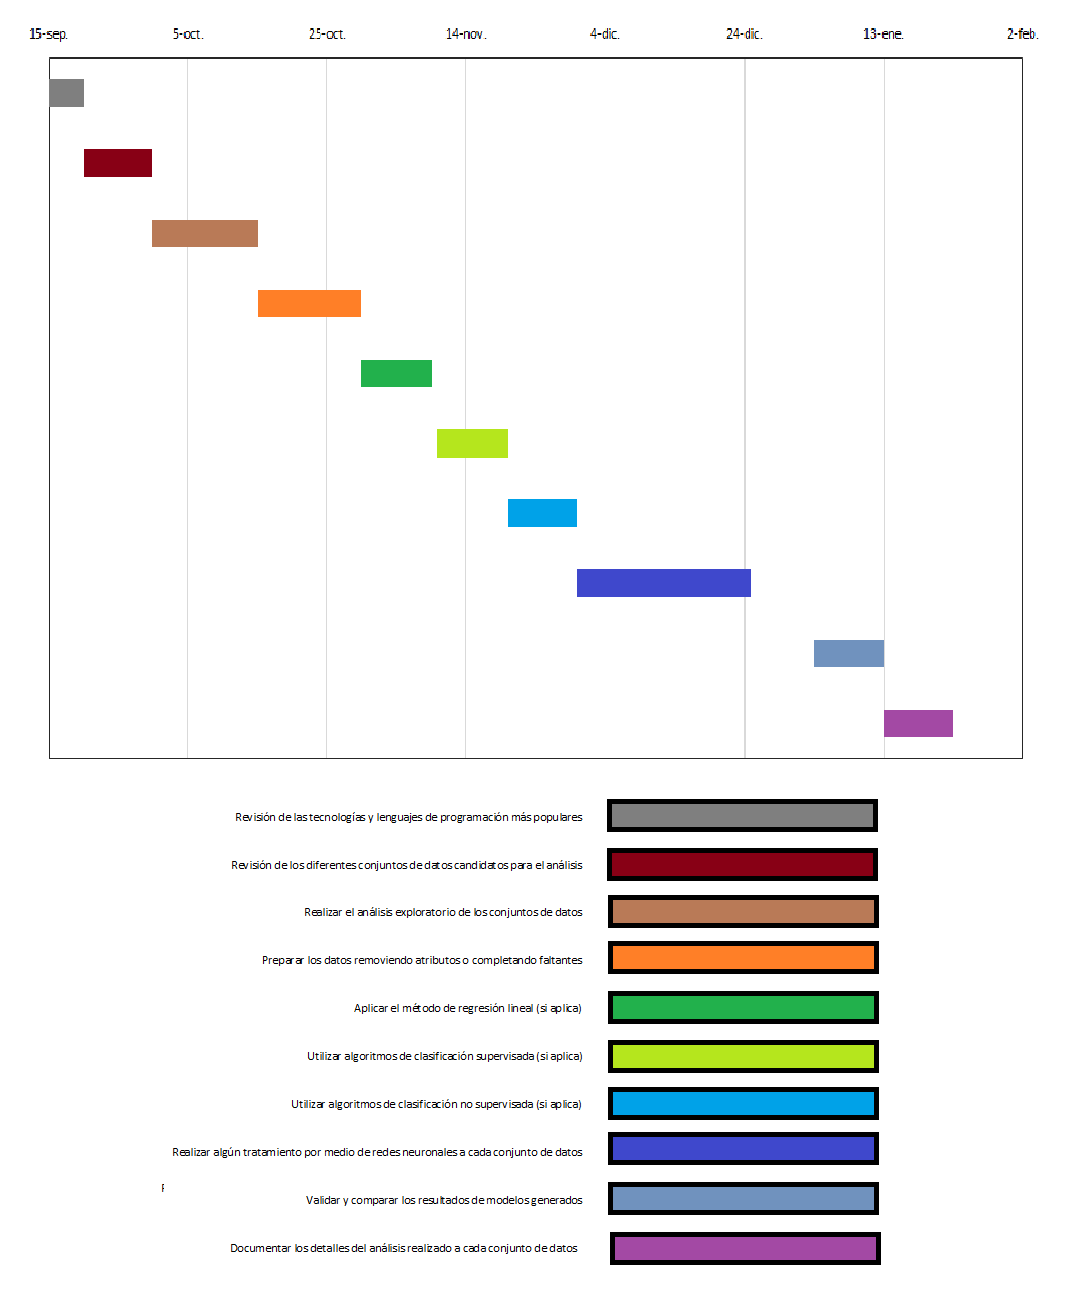
\includegraphics[scale=0.47]{figs/cronograma}
	\caption{Cronograma de actividades de la pasant\'ia} 
	\label{fig:cronograma}
\end{figure}



% Limitacion del problema 
%\begin{center}
\section{ALCANCE Y LIMITACIONES}
\end{center}

\subsection{ALCANCE}

\noindent Este proyecto pretende aportar una soluci\'on de software que se constituya como una fuente de datos confiable, importante y útil para la administración de cultivos en ambientes controlados. Por lo tanto es pertinente aclarar y resaltar que:

\begin{itemize}
	\item Para el desarrollo del prototipo no se incluir\'a la publicaci\'on en tiendas como lo son \textit{Play Store y App Store}.
	\item En condiciones id\'oneas sería de gran valor tener todas las variables ambientales que interactuan directa e indirectamente sobre el objeto de estudio, pero teniendo en cuenta que tanto el rendimiento de la aplicaci\'on  y los costos de infraestructura se podrían ver afectados considerablemente, se recolectara unicamente la informaci\'on que provea alguno de los dispositivos dedicados a esa labor y que est\'en disponibles en el mercado. 
	\item No se har\'a ningún tipo de an\'alisis, clasificación o tratamiento a los datos recolectados ya que el prototipo se limita a la presentaci\'on de la informaci\'on y \'unicamente se realizaran las transformaciones respectivas para cumplir con ese fin.
\end{itemize}

%\lipsum[5]
\subsection{LIMITACIONES}
%\lipsum[6]

\noindent Entre los diversos factores que pueden presentarse en el desarrollo y ejecución de una solución tecnológica; las siguientes son de gran relevancia y alto impacto para la ejecución de este proyecto, por lo tanto es necesario considerar:

\begin{itemize}
	\item \textit{La cobertura y velocidad del canal de comunicaciones.} Teniendo en cuenta que si falla o no funciona adecuadamente; el producto de software no tendrá el resultado y/o el impacto esperado.
	\item \textit{La capacidad de almacenamiento y procesamiento los dispositivos es limitada.} Por lo tanto no se guardaran registros ambientales en la memoria del dispositivo donde se instale el prototipo y la aplicaci\'on sera compatible con los tel\'efonos que se determinen en la fase de diseño e implementaci\'on.
\end{itemize}
 
% Bibliografia
\newpage
\addcontentsline{toc}{section}{REFERENCIAS}
\begin{center}

\vspace{10.5cm}
\singlespace %interlineado 1
%\bibliographystyle{apalike}
%\bibliography{biblio}
\bibliographystyle{IEEEtran}
\bibliography{IEEEabrv,biblio}
\end{center}

% Anexos
%\newpage
%\section*{\begin{center}
%ANEXOS
%\end{center}}
%\addcontentsline{toc}{section}{ANEXOS}

%\section*{A. ANEXO 1}
%\lipsum[1]

%\section*{B. ANEXO 2}
%\lipsum[1]

%\addcontentsline{toc}{section}{ÍNDICE}
\printindex

\end{document}


